% meta.concepts: distributed load
% meta.tags: realistic
% acknowledge: Peter Seiler & Luke Melander graciously shared Spring 2019 course material
% source: 2019 P. Seiler AEM2011 HW 7

\texttt{NOT READY FOR USAGE}
\texttt{THIS PROBLEM/SOLUTION NEEDS TO BE CHECKED.  FOR EXAMPLE "R" SHOULD BE 740 FT, NOT 500 ft"}


Hoover dam, built in 1936 holds the Lake Mead in Nevada. The structure is 726 ft high and has an arc length
of 1,244 ft. In order to determine how strong the dam is, you have to determine the force applied by the water
on the dam wall. Assume that the dam is shaped like a circular arc with a radius of curvature of 740 ft. The
height of the water is 500 ft. Assuming that the force applied by the water is perpendicular to the wall, find
the X and Y component of the force applied by the water on the dam in the coordinate system shown (Z
component will be zero)

\begin{figure}[ht!]
  \centering
  \includegraphics[height=1.5in]{figa.png}
  \includegraphics[height=1.5in]{figb.png}
  \caption*{(left) Hoover Dam.  (right) Schematic diagram of the dam.}
\end{figure}

\iftoggle{flagSoln}{%
\vspace{.5cm}
\rule{\textwidth}{.4pt}
\vspace{.5cm}
\textbf{Solution:}
\begin{figure}[ht!]
  \centering
  \includegraphics[width=0.9\textwidth,
	           height=0.3\textheight,
		   keepaspectratio]{solna.png}
  \includegraphics[width=0.9\textwidth,
	           height=0.3\textheight,
		   keepaspectratio]{solnb.png}
  \includegraphics[width=0.9\textwidth,
	           height=0.3\textheight,
		   keepaspectratio]{solnc.png}
\end{figure}
}{%
}%
